\documentclass[
11pt, % The default document font size, options: 10pt, 11pt, 12pt
%codirector, % Uncomment to add a codirector to the title page
]{charter} 


% El títulos de la memoria, se usa en la carátula y se puede usar el cualquier lugar del documento con el comando \ttitle
\titulo{Sistema multi-agente basado en modelos de lenguaje locales y generación aumentada por recuperación (RAG) para la asistencia segura en asesoría financiera}

% Nombre del posgrado, se usa en la carátula y se puede usar el cualquier lugar del documento con el comando \degreename
\posgrado{Carrera de Especialización en Inteligencia Artificial}

% Tu nombre, se puede usar el cualquier lugar del documento con el comando \authorname
% IMPORTANTE: no omitir titulaciones ni tildación en los nombres, también se recomienda escribir los nombres completos (tal cual los tienen en su documento)
\autor{Nailé Paola Cartalá}

% El nombre del director y co-director, se puede usar el cualquier lugar del documento con el comando \supname y \cosupname y \pertesupname y \pertecosupname
\director{A Definir}
\pertenenciaDirector{FIUBA} 
% \codirector{} % para que aparezca en la portada se debe descomentar la opción codirector en los parámetros de documentclass
\pertenenciaCoDirector{FIUBA}

% Nombre del cliente, quien va a aprobar los resultados del proyecto, se puede usar con el comando \clientename y \empclientename
\cliente{Silvina Mengarelli}
\empresaCliente{ULT Finance}
 
\fechaINICIO{3 de marzo de 2026}		%Fecha de inicio de la cursada de GdP \fechaInicioName
\fechaFINALPlan{21 de abril de 2026} 	%Fecha de final de cursada de GdP
\fechaFINALTrabajo{15 de mayo de 2024}	%Fecha de defensa pública del trabajo final


\begin{document}

\maketitle
\thispagestyle{empty}
\pagebreak


\thispagestyle{empty}
{\setlength{\parskip}{0pt}
\tableofcontents{}
}
\pagebreak


\section*{Registros de cambios}
\label{sec:registro}

\begin{table}[ht]
\label{tab:registro}
\centering
\begin{tabularx}{\linewidth}{@{}|c|X|c|@{}}
\hline
\rowcolor[HTML]{C0C0C0} 
Revisión & \multicolumn{1}{c|}{\cellcolor[HTML]{C0C0C0}Detalles de los cambios realizados} & Fecha      \\ \hline
0      & Creación del documento                                 &\fechaInicioName \\ \hline
1      & Se completa hasta el punto 5 inclusive                 & 15 de marzo de 2026 \\ \hline
2      & Se completa hasta el punto 9 inclusive                 & 23 de marzo de 2026 \\ \hline
3      & Se completa hasta el punto 12 inclusive                & 7 de abril de 2026 \\ \hline
%4      & Se completa el plan	                                 & {día} de {mes} de 202X \\ \hline

% Si hay más correcciones pasada la versión 4 también se deben especificar acá

\end{tabularx}
\end{table}

\pagebreak

\section*{Acta de constitución del proyecto}
\label{sec:acta}

\begin{flushright}
Buenos Aires, \fechaInicioName
\end{flushright}

\vspace{2cm}

Por medio de la presente se acuerda con \authorname\hspace{1px} que su Trabajo Final de la \degreename\hspace{1px} se titulará ``\ttitle'' y consistirá en el desarrollo de un asistente virtual financiero seguro mediante una arquitectura multi-agente, modelos de lenguaje locales (open-weights) y generación aumentada por recuperación (RAG). El trabajo tendrá un presupuesto preliminar estimado de 600 horas y un costo estimado de \$ 0 (al utilizar herramientas de código abierto e infraestructura computacional propia), con fecha de inicio el \fechaInicioName\hspace{1px} y fecha de presentación pública el \fechaFinalName.

Se adjunta a esta acta la planificación inicial.

\vfill

% Esta parte se construye sola con la información que hayan cargado en el preámbulo del documento y no debe modificarla
\begin{table}[ht]
\centering
\begin{tabular}{ccc}
\begin{tabular}[c]{@{}c@{}}Dr. Ing. Ariel Lutenberg \\ Director posgrado FIUBA\end{tabular} & \hspace{2cm} & \begin{tabular}[c]{@{}c@{}}\clientename \\ \empclientename \end{tabular} \vspace{2.5cm} \\ 
\multicolumn{3}{c}{\begin{tabular}[c]{@{}c@{}} \supname \\ Director del Trabajo Final\end{tabular}} \vspace{2.5cm} \\
\end{tabular}
\end{table}




\section{1. Descripción técnica-conceptual del proyecto a realizar}
\label{sec:descripcion}

En la industria de la gestión patrimonial (wealth management), los asesores financieros invierten una cantidad desproporcionada de su tiempo en tareas administrativas y de cumplimiento normativo, tales como la transcripción de reuniones, el análisis de métricas de portafolios y la redacción de reportes. Si bien la adopción actual de herramientas de Inteligencia Artificial (IA) generativa pública ofrece una vía para automatizar estas tareas, su uso presenta un riesgo crítico en este sector. El estado del arte obliga a las instituciones a elegir entre la eficiencia de la IA centralizada y la estricta privacidad de los datos, ya que enviar información de identificación personal (PII) o datos financieros a servidores de terceros viola las estrictas normativas de confidencialidad y regulaciones financieras (como las de la SEC). 

Para abordar esta problemática, el presente proyecto, desarrollado como un emprendimiento personal enfocado en el sector Fintech, propone el desarrollo de un asistente virtual financiero basado en una arquitectura segura. La solución consiste en un sistema orquestado por múltiples agentes inteligentes que utilizan Modelos Fundacionales ejecutados en hardware local (Edge AI o servidores on-premise). El sistema integra procesamiento de lenguaje natural (NLP) para estructurar notas de reuniones y análisis automatizado de portafolios de inversión. Todo esto se unifica mediante una interfaz conversacional impulsada por un motor de Generación Aumentada por Recuperación (RAG), que permite realizar consultas cruzadas sobre el historial de clientes sin que un solo dato salga de la infraestructura local.

La propuesta de valor radica en ofrecer la máxima eficiencia operativa bajo un paradigma de ``Confianza Cero'' (Zero-Trust). Lo que distingue a este proyecto de otras soluciones comerciales SaaS es la garantía absoluta de privacidad de los datos mediante el uso de modelos de lenguaje de pesos abiertos (open-weights), sumado a una trazabilidad completa de las decisiones algorítmicas mediante herramientas determinísticas (Tool Calling).

En la figura \ref{fig:diagBloques} se presenta el diagrama en bloques del sistema. Se observa que la arquitectura se divide en cuatro capas principales. En la parte superior, la capa de cliente captura las interacciones. Estas se derivan a una capa de servicios asíncrona basada en colas (SQLite) que previene el bloqueo del servidor. Posteriormente, la capa de inteligencia artificial, comandada por un Agente Enrutador, deriva las tareas a sub-agentes especializados que se comunican con el motor de inferencia local. Finalmente, la capa inferior gestiona el almacenamiento estructurado (SQL) y el conocimiento semántico (Vector DB).

\begin{figure}[htpb]
\centering 
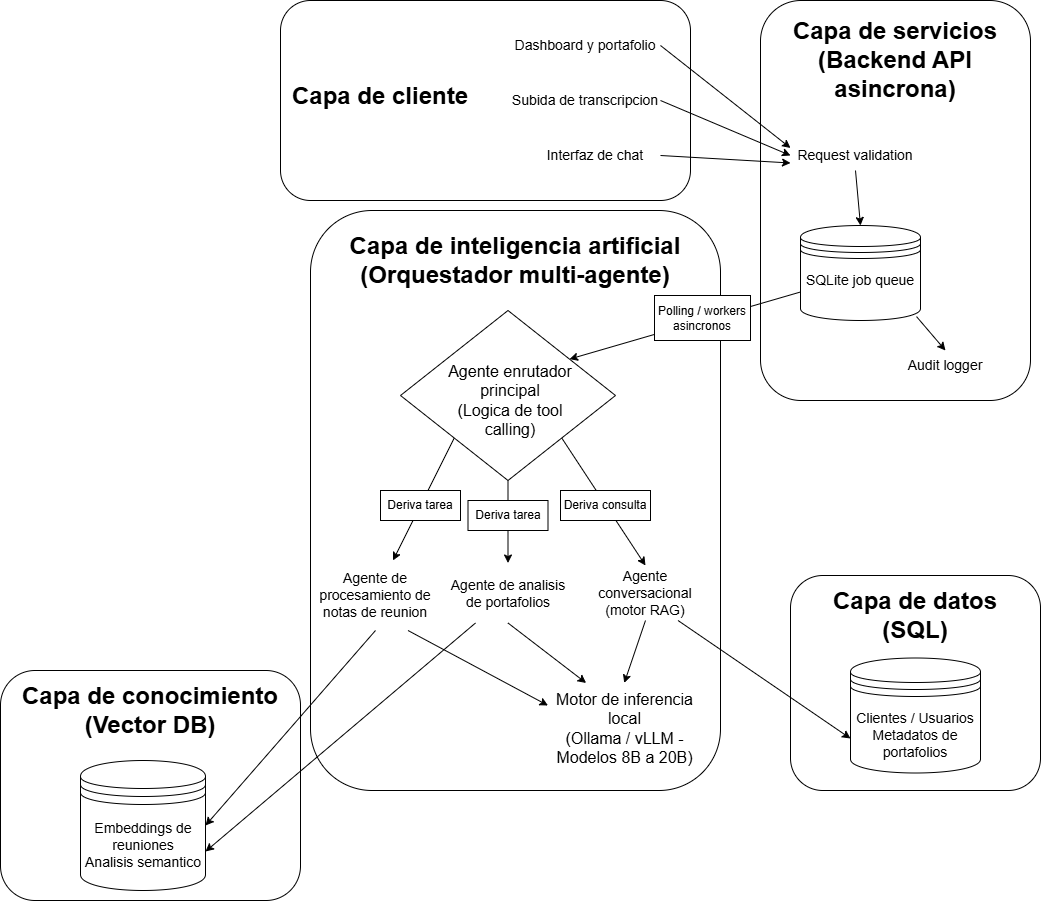
\includegraphics[width=.85\textwidth]{./Figuras/diagBloques.png}
\caption{Diagrama en bloques de la arquitectura multi-agente propuesta.}
\label{fig:diagBloques}
\end{figure}

\section{2. Identificación y análisis de los interesados}
\label{sec:interesados}

\begin{table}[ht]
%\caption{Identificación de los interesados}
%\label{tab:interesados}
\begin{tabularx}{\linewidth}{@{}|l|X|X|l|@{}}
\hline
\rowcolor[HTML]{C0C0C0} 
Rol           & Nombre y Apellido & Organización 	& Puesto 	\\ \hline
Cliente       & \clientename      &\empclientename	&    CEO    	\\ \hline
Responsable   & \authorname       & FIUBA        	& Alumno 	\\ \hline
Orientador    & \supname	      & \pertesupname 	& Director del Trabajo Final \\ \hline
\end{tabularx}
\end{table}

A continuación, se detallan las principales características y expectativas de cada uno de los interesados en el proyecto:

\begin{itemize}
    \item \textbf{Cliente (\clientename):} es un sector altamente regulado y riguroso. Valora por sobre todo la privacidad de los datos (arquitectura Zero-Trust) y el cumplimiento normativo (regulaciones de la SEC). Su principal expectativa es que el sistema reduzca drásticamente el tiempo invertido en tareas administrativas sin sacrificar la seguridad de la información confidencial de sus propios clientes.
    
    \item \textbf{Responsable (\authorname):} es la encargada de la investigación, el diseño de la arquitectura y el desarrollo integral del código (orquestación de agentes, configuración del motor RAG y bases de datos). Dado que este proyecto se realiza en paralelo con otras actividades profesionales, el desarrollo se planificará con una dedicación parcial estructurada y tendrá un enfoque de avance iterativo e incremental.
    
    \item \textbf{Orientador (\supname):} profesional con titulación de posgrado y sólida experiencia técnica en Inteligencia Artificial o Arquitectura de Software. Su rol principal será guiar metodológicamente el proyecto, validar las decisiones arquitectónicas del sistema multi-agente, aportar retroalimentación sobre la calidad de las métricas de evaluación del modelo (RAG) y asegurar que el trabajo cumpla con los estándares académicos exigidos por la Universidad.
\end{itemize}

\section{3. Propósito del proyecto}
\label{sec:proposito}

Automatizar y asegurar el procesamiento de información confidencial en el ámbito de la asesoría financiera mediante el desarrollo de un sistema multi-agente. Este sistema busca reducir la carga administrativa de los profesionales y garantizar la privacidad absoluta de los datos a través de la ejecución local de modelos de lenguaje, para así cumplir con las estrictas normativas regulatorias del sector.

\section{4. Alcance del proyecto}
\label{sec:alcance}

El proyecto incluye:
\begin{itemize}
    \item Desarrollo de un orquestador multi-agente (agente enrutador, agente conversacional, agente de análisis de portafolios y agente de procesamiento de notas).
    \item Integración de modelos de lenguaje de pesos abiertos (open-weights) ejecutados de forma local para garantizar la privacidad.
    \item Implementación de un motor de Generación Aumentada por Recuperación (RAG) conectado a una base de datos vectorial para el historial de reuniones.
    \item Creación de un dataset sintético paramétrico con perfiles de clientes, portafolios y transcripciones de reuniones para la validación del sistema.
    \item Diseño de una arquitectura de servicios asíncrona basada en colas de tareas con base de datos SQLite.
\end{itemize}

El presente proyecto no incluye:
\begin{itemize}
    \item Integración directa con bases de datos en producción o interfaces de programación de aplicaciones (API) de plataformas financieras comerciales reales (como Redtail CRM o Albridge).
    \item Despliegue del sistema en servidores en la nube orientados a usuarios finales en un entorno de producción.
    \item Desarrollo de aplicaciones móviles nativas para el acceso al asistente virtual.
\end{itemize}

\section{5. Supuestos del proyecto}
\label{sec:supuestos}

Para el desarrollo del presente proyecto se supone que:

\begin{itemize}
    \item Se dispondrá de acceso a hardware con capacidad de cómputo y memoria VRAM suficiente (tarjetas gráficas dedicadas o servicios en la nube temporal) para la inferencia local de modelos de lenguaje de entre 8B y 20B parámetros con tiempos de respuesta aceptables.
    \item Será factible desarrollar un pipeline procedural capaz de generar un dataset sintético representativo (que incluya perfiles de clientes, portafolios y transcripciones de reuniones) que permita entrenar y validar el sistema sin infringir normativas de confidencialidad.
    \item Los frameworks de orquestación multi-agente de código abierto seleccionados (como PydanticAI o LangChain) mantendrán soporte y estabilidad durante el ciclo de vida del desarrollo.
    \item La arquitectura asíncrona propuesta mediante colas de trabajo en SQLite será suficiente para gestionar la concurrencia esperada en un entorno de prototipo, sin requerir la implementación inicial de gestores de colas más complejos (como Celery o RabbitMQ).
    \item Se contará con la disponibilidad periódica del experto del dominio (cliente) para la validación cualitativa de las respuestas generadas por los agentes y la verificación del cumplimiento de las reglas de negocio financieras.
    \item El modelo de incrustación (embeddings) seleccionado para la base de datos vectorial logrará una precisión semántica suficiente para que el motor RAG recupere el contexto relevante sin inducir alucinaciones críticas en las respuestas.
\end{itemize}

\section{6. Product backlog}
\label{sec:backlog}

El Product Backlog se ha organizado en cuatro épicas fundamentales que agrupan las funcionalidades clave del sistema multi-agente. 

La ponderación de las historias de usuario se realizó utilizando Story Points (SP) basados en la serie de Fibonacci (1, 2, 3, 5, 8, 13). El criterio para el cálculo de los SP consiste en asignar un valor del 1 al 5 a tres variables independientes: dificultad temporal (tiempo estimado de implementación), complejidad técnica (cantidad de dependencias del código) e incertidumbre (nivel de experiencia previa requerida). La suma aritmética de estas tres variables se aproxima al número superior más cercano dentro de la sucesión de Fibonacci para obtener el valor final asignado a la historia.

Las épicas y sus respectivas historias, incluyendo la justificación de sus prioridades, se detallan a continuación:

\begin{itemize}
  \item \textbf{\'{E}pica 1: generación y gestión de datos sintéticos}
    \begin{itemize}
      \item HU1: como desarrollador, quiero generar un dataset sintético de clientes y portafolios para entrenar y validar el sistema sin comprometer datos reales confidenciales. Prioridad alta, ya que sin datos de prueba estructurados no es posible construir ni validar el resto de los módulos del sistema. 5 SP.
      \item HU2: como desarrollador, quiero simular transcripciones de reuniones financieras con diferentes niveles de complejidad técnica para probar la robustez del agente de procesamiento de notas. Prioridad alta, porque representa la entrada de datos fundamental para iniciar el flujo de procesamiento de lenguaje natural. 3 SP.
    \end{itemize}
  \item \textbf{\'{E}pica 2: procesamiento y análisis de notas de reuniones}
    \begin{itemize}
      \item HU3: como asesor financiero, quiero subir transcripciones de reuniones al sistema para que el agente extraiga automáticamente los puntos clave, entidades y recomendaciones. Prioridad alta, pues constituye el núcleo de la asistencia automatizada para reducir la carga administrativa. 8 SP.
      \item HU4: como oficial de cumplimiento, quiero que el sistema analice las notas de las reuniones y aplique verificaciones normativas predefinidas para identificar posibles riesgos regulatorios. Prioridad media, porque aporta un gran valor de auditoría pero el sistema conversacional puede funcionar en su primera iteración sin estas reglas activadas. 5 SP.
    \end{itemize}
  \item \textbf{\'{E}pica 3: análisis automatizado de portafolios}
    \begin{itemize}
      \item HU5: como asesor financiero, quiero cargar datos tabulares de un portafolio de inversión para obtener un reporte automatizado de métricas de riesgo y alocación de activos. Prioridad alta, ya que conforma la funcionalidad central y bloqueante del módulo de inversiones. 8 SP.
      \item HU6: como asesor financiero, quiero que el agente compare el rendimiento del portafolio actual con benchmarks para fundamentar mis estrategias de inversión. Prioridad media, porque optimiza el análisis cualitativo pero no impide el cálculo de riesgo matemático básico. 5 SP.
    \end{itemize}
  \item \textbf{\'{E}pica 4: interfaz conversacional y motor RAG}
    \begin{itemize}
      \item HU7: como asesor financiero, quiero interactuar con un chatbot en lenguaje natural para realizar consultas rápidas y que el Agente Enrutador derive mi pedido al sub-agente correspondiente mediante Tool Calling. Prioridad alta, porque es la única interfaz de interacción habilitada para que el usuario final utilice el sistema. 8 SP.
      \item HU8: como asesor financiero, quiero que el chatbot recupere información histórica de reuniones pasadas mediante búsqueda semántica (RAG) para preparar mis próximas interacciones con clientes. Prioridad alta, porque representa el mayor diferenciador tecnológico del sistema propuesto al dotar de memoria a largo plazo a la inteligencia artificial. 13 SP.
    \end{itemize}
\end{itemize}

\section{7. Criterios de aceptación de historias de usuario}
\label{sec:criteriosAceptacion}

Los siguientes criterios establecen las condiciones medibles y verificables que deben cumplirse para dar por finalizada cada historia de usuario:

\begin{itemize}
  \item \textbf{\'{E}pica 1: generación y gestión de datos sintéticos}
    \begin{itemize}
      \item Criterios de aceptación HU1:
        \begin{enumerate}
          \item El dataset debe contener al menos 100 perfiles de clientes simulados.
          \item Los datos generados deben exportarse en formato estructurado (CSV/JSON).
          \item Los registros no deben contener ninguna información de identificación personal (PII) real.
        \end{enumerate}
      \item Criterios de aceptación HU2:
        \begin{enumerate}
          \item Se deben generar al menos 50 transcripciones de prueba.
          \item El 20\% de las transcripciones deben incluir terminología financiera ambigua intencional.
          \item Los archivos generados deben almacenarse en formato de texto plano (.txt).
        \end{enumerate}
    \end{itemize}
    
  \item \textbf{\'{E}pica 2: procesamiento y análisis de notas de reuniones}
    \begin{itemize}
      \item Criterios de aceptación HU3:
        \begin{enumerate}
          \item El sistema debe procesar un archivo de texto en un tiempo menor a 30 segundos.
          \item La salida debe extraer de forma estructurada al menos entidades, fechas y recomendaciones.
          \item El resultado debe devolverse en formato JSON para su persistencia en la base de datos.
        \end{enumerate}
      \item Criterios de aceptación HU4:
        \begin{enumerate}
          \item El sistema debe marcar con una bandera de alerta los documentos que infrinjan normativas simuladas de la SEC.
          \item Se debe generar un registro de auditoría en la base de datos por cada revisión completada.
          \item La precisión cualitativa de detección de violaciones debe ser evaluada como aceptable por el experto del dominio.
        \end{enumerate}
    \end{itemize}
    
  \item \textbf{\'{E}pica 3: análisis automatizado de portafolios}
    \begin{itemize}
      \item Criterios de aceptación HU5:
        \begin{enumerate}
          \item El agente debe ingerir correctamente archivos CSV de hasta 5 MB.
          \item El reporte generado debe calcular e incluir al menos tres métricas de riesgo financiero.
          \item El resultado del análisis debe visualizarse claramente en la interfaz de usuario.
        \end{enumerate}
      \item Criterios de aceptación HU6:
        \begin{enumerate}
          \item El análisis debe integrar al menos un índice de referencia sintético para la comparación.
          \item El agente debe generar una justificación en texto natural que explique las desviaciones de rendimiento.
          \item Las operaciones matemáticas de comparación no deben presentar errores de cálculo.
        \end{enumerate}
    \end{itemize}
    
  \item \textbf{\'{E}pica 4: interfaz conversacional y motor RAG}
    \begin{itemize}
      \item Criterios de aceptación HU7:
        \begin{enumerate}
          \item La interfaz web debe poseer una ventana de chat funcional.
          \item El Agente Enrutador debe invocar correctamente las herramientas (Tool Calling) según la intención del usuario.
          \item El sistema debe gestionar el historial para mantener el contexto durante al menos cinco interacciones continuas.
        \end{enumerate}
      \item Criterios de aceptación HU8:
        \begin{enumerate}
          \item El sistema debe instanciar y consultar una base de datos vectorial local.
          \item Las respuestas generadas por el modelo deben incluir al menos una referencia al documento recuperado.
          \item El motor RAG debe combinar la recuperación de metadatos SQL con la similitud de cosenos en el espacio vectorial.
        \end{enumerate}
    \end{itemize}
\end{itemize}

\section{8. Fases de CRISP-DM}

Al tratarse de un proyecto intensivo en datos e inteligencia artificial, la planificación del ciclo de vida se basa en la metodología CRISP-DM adaptada a enfoques ágiles:

\begin{enumerate}
  \item \textbf{Comprensión del negocio:} reducir la carga administrativa y de cumplimiento normativo de los asesores financieros para garantizar la confidencialidad mediante arquitectura Zero-Trust. La métrica de éxito esperada es la automatización exitosa de tareas operativas que normalmente toman horas, para reducirlas a segundos.
  \item \textbf{Comprensión de los datos:} se trabajarán tres fuentes de datos sintéticos generados ad-hoc. Datos tabulares estructurados (perfiles de clientes), datos financieros (CSV de portafolios) y datos no estructurados de tipo texto (cientos de documentos de transcripciones de reuniones).
  \item \textbf{Preparación de los datos:} incluirá la limpieza de texto, normalización de formatos numéricos y, críticamente, la fragmentación (chunking) de los documentos de texto para la generación de incrustaciones (embeddings) vectoriales.
  \item \textbf{Modelado:} el problema se enfoca en tareas de Procesamiento de Lenguaje Natural (NLP) y Generación Aumentada por Recuperación (RAG). Se emplearán modelos fundacionales de pesos abiertos (de 8B a 20B parámetros) ejecutados localmente y orquestados mediante frameworks de agentes (como PydanticAI).
  \item \textbf{Evaluación del modelo:} se priorizará una validación cualitativa (Human-in-the-Loop) por parte del experto del dominio (cliente). Adicionalmente, se medirán los tiempos de latencia en la inferencia y se auditará la calidad de recuperación del contexto en el motor RAG.
  \item \textbf{Despliegue del modelo:} la solución se empaquetará utilizando una interfaz web y un backend asíncrono (FastAPI) acoplado a colas de tareas en SQLite, pensado para ejecutarse de forma local u on-premise.
\end{enumerate}

\section{9. Desglose del trabajo en tareas}
\label{sec:wbs}

A continuación, se desglosan las Historias de Usuario (HU) en tareas técnicas específicas, accionables y con una estimación temporal acotada para facilitar la posterior planificación de los Sprints:

\begin{table}[htpb]
\centering
\begin{tabularx}{\linewidth}{@{}|c|X|c|c|@{}}
\hline
\rowcolor[HTML]{C0C0C0}
HU & Tarea técnica & Estimación & Prioridad \\ \hline
HU1 & Programar script de generación de perfiles de clientes & 4 h & Alta \\ \hline
HU1 & Desarrollar generador de datos de portafolios en CSV & 6 h & Alta \\ \hline
HU2 & Crear prompts de generación de diálogos para el LLM & 3 h & Media \\ \hline
HU2 & Ejecutar generación masiva de transcripciones sintéticas & 5 h & Alta \\ \hline
HU3 & Implementar endpoint asíncrono para ingesta de archivos & 4 h & Alta \\ \hline
HU3 & Configurar prompt de extracción estructurada en JSON & 6 h & Alta \\ \hline
HU4 & Definir catálogo de reglas de cumplimiento simuladas & 3 h & Baja \\ \hline
HU4 & Implementar validador normativo en pipeline de notas & 5 h & Media \\ \hline
HU5 & Desarrollar módulo parser de archivos CSV de portafolios & 4 h & Alta \\ \hline
HU5 & Programar cálculos de métricas de riesgo en Python & 7 h & Alta \\ \hline
HU6 & Generar estructura de datos para benchmarks sintéticos & 3 h & Baja \\ \hline
HU6 & Implementar lógica de comparación de rendimientos & 5 h & Media \\ \hline
HU7 & Desarrollar interfaz de usuario del chatbot (Frontend) & 6 h & Alta \\ \hline
HU7 & Implementar Agente Enrutador con Tool Calling & 8 h & Alta \\ \hline
HU8 & Configurar base de datos vectorial local y embeddings & 6 h & Alta \\ \hline
HU8 & Programar pipeline de fragmentación e ingesta (chunking) & 5 h & Alta \\ \hline
HU8 & Desarrollar flujo de recuperación y generación (RAG) & 8 h & Alta \\ \hline
\end{tabularx}
\end{table}

\section{10. Planificación de sprints}
\label{sec:sprints}

La planificación del proyecto contempla un total estimado de 600 horas de trabajo. Se ha definido un esquema de 12 sprints de dos semanas de duración cada uno para garantizar un avance iterativo. De acuerdo con las metodologías ágiles, la velocidad del equipo se mide mediante la asignación de Story Points basada en la serie de Fibonacci. Las tareas técnicas requieren aproximadamente 40 a 45 horas por sprint, mientras que el tiempo restante se destina a investigación, pruebas, documentación y reuniones.

\begin{table}[htpb]
\centering
\caption{Planificación de sprints y asignación de tareas}
\begin{tabularx}{\linewidth}{@{}|l|l|X|c|l|c|@{}}
\hline
\rowcolor[HTML]{C0C0C0}
Sprint & HU o fase & Tarea & Horas / SP & Responsable & \% Completado \\ \hline
Sprint 0 & Planificación & Redacción del plan de proyecto y cronograma & 15 h & Alumno & 100\% \\ \hline
Sprint 1 & Arquitectura & Configuración del entorno y bases de datos & 40 h & Alumno & 0\% \\ \hline
Sprint 2 & HU1 & Generación de dataset sintético de perfiles & 40 h / 5 SP & Alumno & 0\% \\ \hline
Sprint 3 & HU2 & Simulación masiva de transcripciones & 42 h / 3 SP & Alumno & 0\% \\ \hline
Sprint 4 & HU3 & Extracción estructurada de entidades (JSON) & 45 h / 8 SP & Alumno & 0\% \\ \hline
Sprint 5 & HU4 & Desarrollo del validador normativo SEC & 40 h / 5 SP & Alumno & 0\% \\ \hline
Sprint 6 & HU5 & Parser y métricas de riesgo para portafolios & 45 h / 8 SP & Alumno & 0\% \\ \hline
Sprint 7 & HU6 & Lógica de comparación con benchmarks & 40 h / 5 SP & Alumno & 0\% \\ \hline
Sprint 8 & HU8 & Pipeline de fragmentación y embeddings local & 45 h / 8 SP & Alumno & 0\% \\ \hline
Sprint 9 & HU8 & Flujo de recuperación y motor RAG & 45 h / 13 SP & Alumno & 0\% \\ \hline
Sprint 10 & HU7 & Interfaz de usuario e integración Tool Calling & 45 h / 8 SP & Alumno & 0\% \\ \hline
Sprint 11 & Validación & Pruebas finales y ajustes del sistema & 40 h & Alumno & 0\% \\ \hline
Sprint 12 & Cierre & Redacción de la memoria y preparación de la defensa & 118 h & Alumno & 0\% \\ \hline
\end{tabularx}
\end{table}


\section{11. Diagrama de Gantt}
\label{sec:gantt}

El siguiente diagrama de Gantt ilustra la distribución temporal de los 12 sprints a lo largo de los meses de ejecución del proyecto. Se diferencian las etapas de planificación inicial, el desarrollo técnico iterativo y las fases finales de redacción de la memoria y defensa pública.

\begin{figure}[htpb]
\centering 
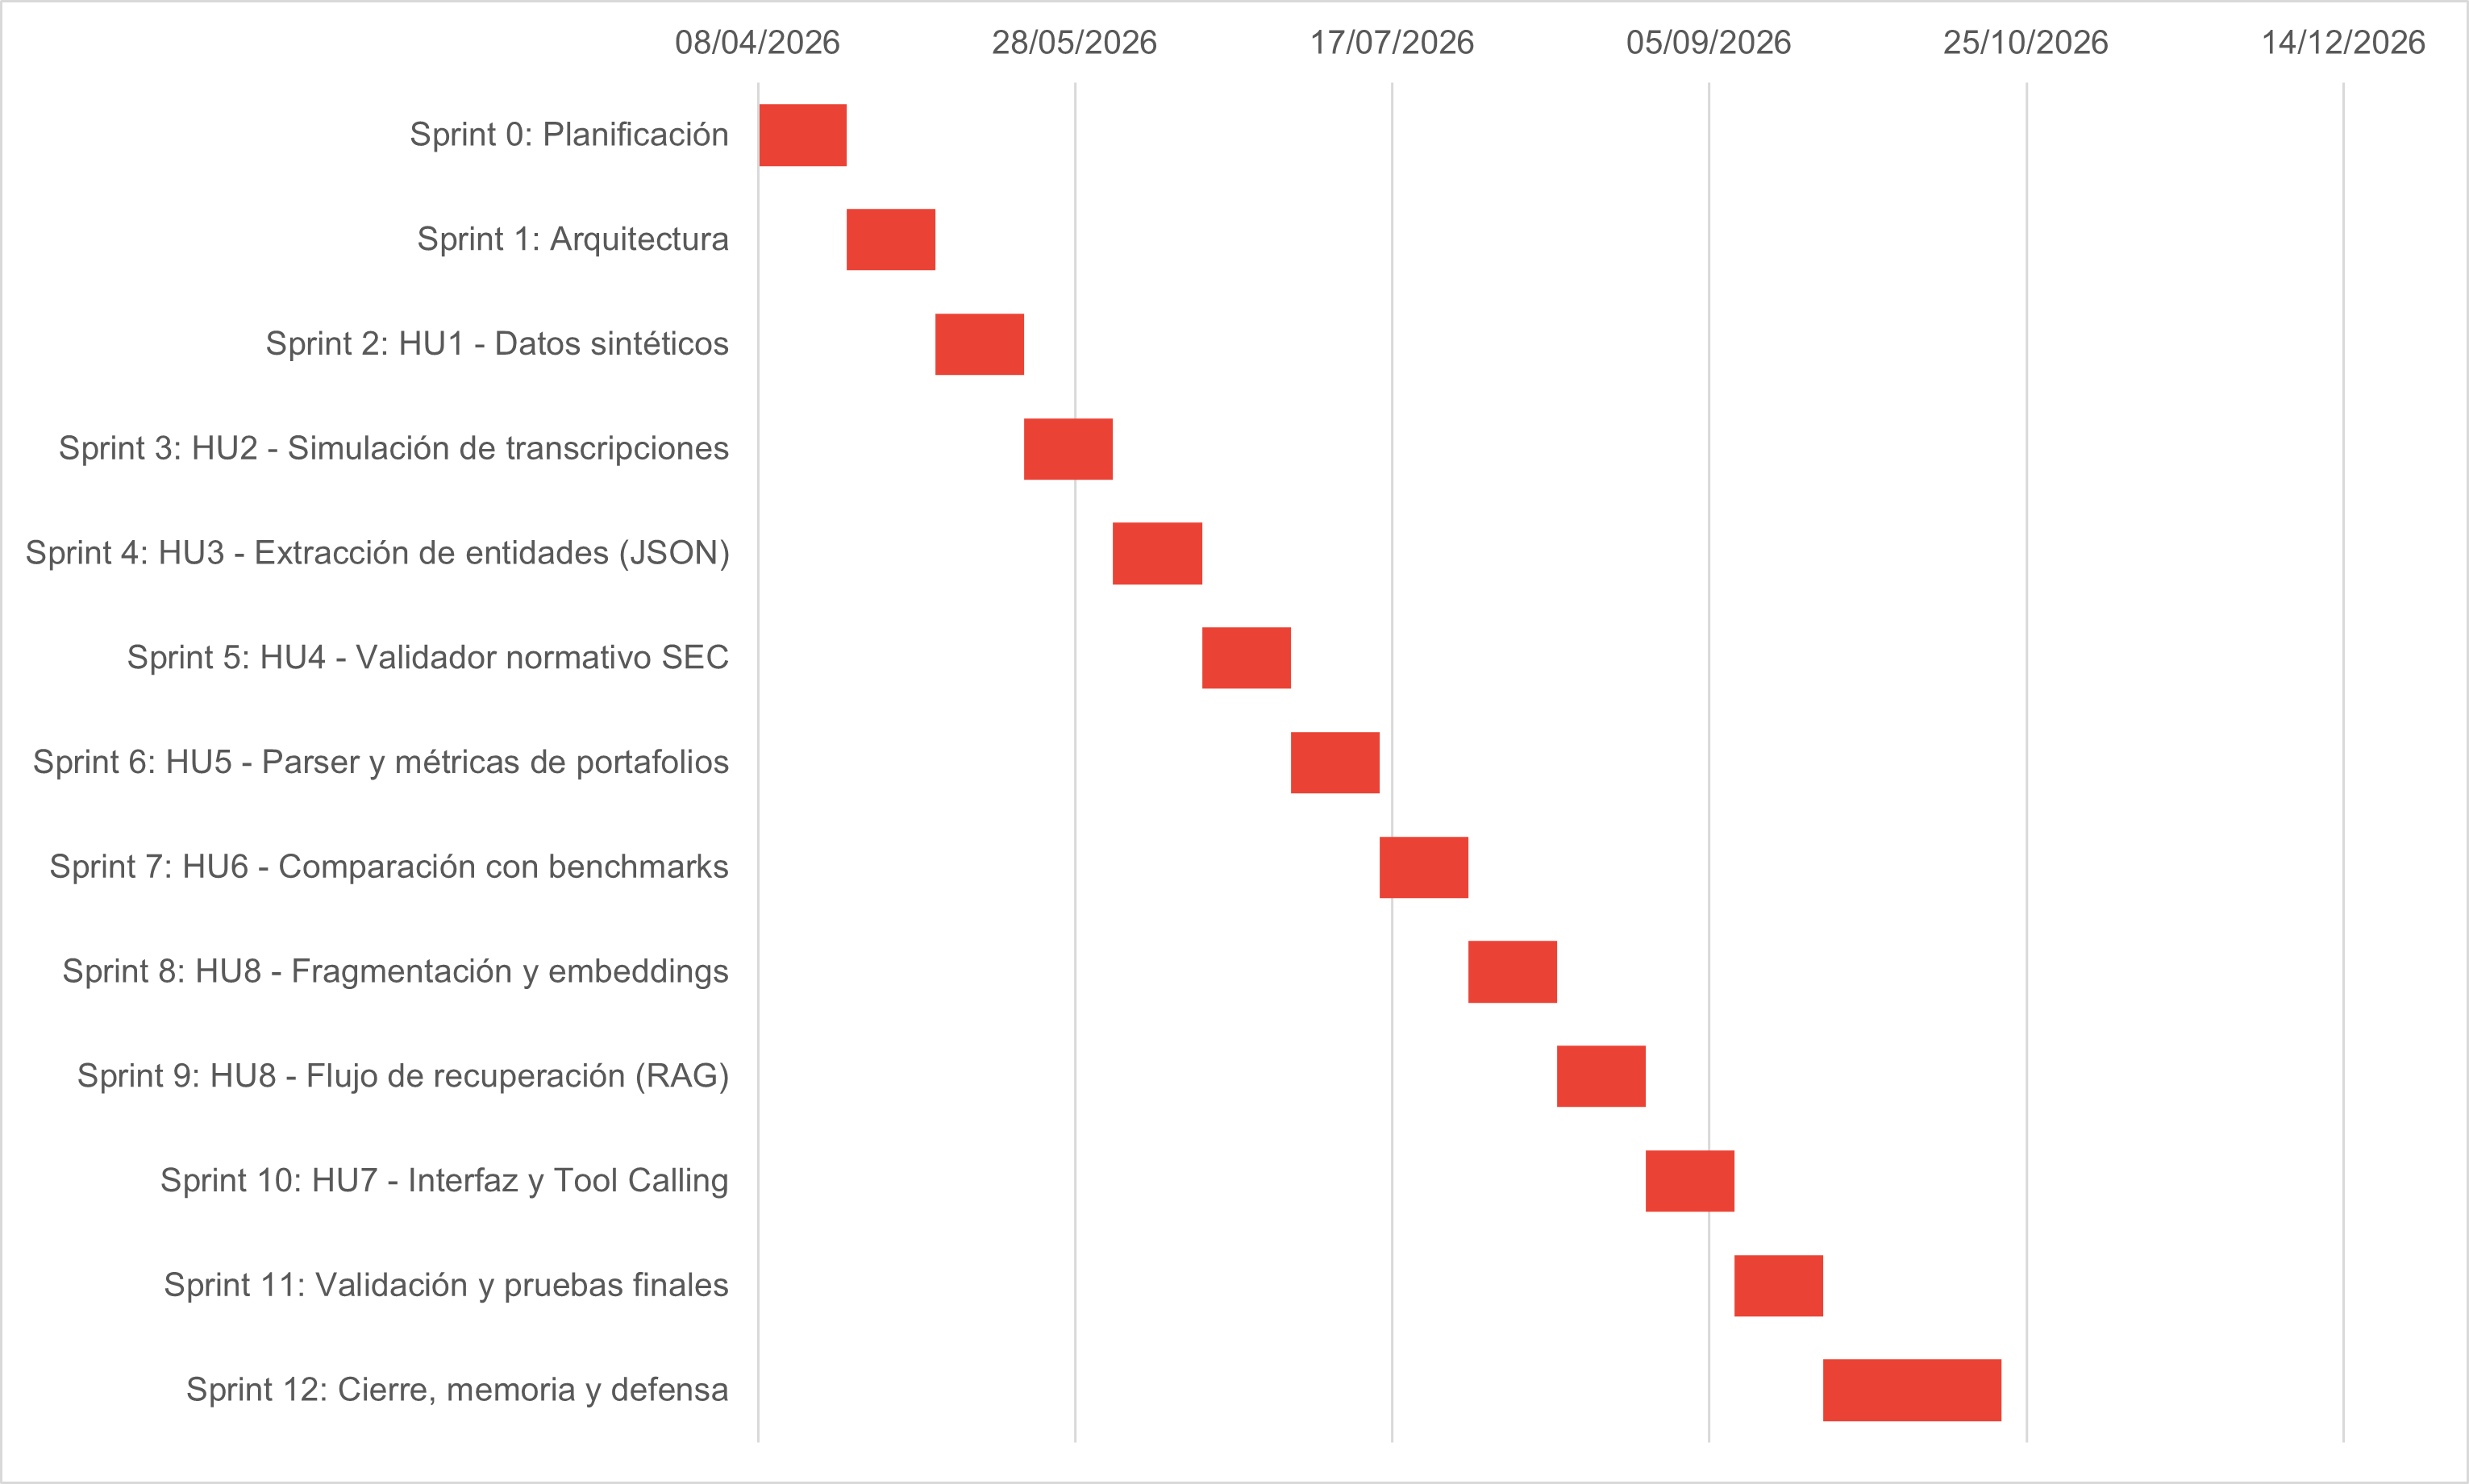
\includegraphics[width=.95\textwidth]{./Figuras/Gantt-2.png}
\caption{Diagrama de Gantt con la planificación temporal de los sprints.}
\label{fig:gantt}
\end{figure}


\section{12. Gobernanza de datos}
\label{sec:gobernanza}

El proyecto integra un análisis constante de la gobernanza de datos desde las fases iniciales del ciclo de vida para garantizar la calidad y la viabilidad legal del producto. El concepto de calidad se define, bajo los lineamientos de la norma ISO 9000, como el nivel en que las características del sistema satisfacen los requerimientos operativos y de seguridad.

\subsection{Cumplimiento normativo}
El sistema procesa información del sector financiero, por lo que el cumplimiento normativo es el eje central de su diseño. Se establece que:
\begin{itemize}
  \item la arquitectura Zero-Trust y el uso de modelos open-weights locales previenen la fuga de datos hacia servidores de terceros.
  \item esta estrategia garantiza el cumplimiento de la Ley 25.326 de Protección de Datos Personales en Argentina y se alinea con los estándares de confidencialidad de la SEC para la gestión de información de identificación personal (PII).
  \item los datos de entrenamiento y prueba se limitan a un dataset sintético autogenerado que anula cualquier riesgo de violar acuerdos de confidencialidad.
\end{itemize}

\subsection{Ética en el uso de inteligencia artificial}
El diseño del sistema asume la responsabilidad de mitigar posibles riesgos éticos derivados del uso de modelos generativos:
\begin{itemize}
  \item para evitar la manipulación o la desinformación financiera mediante alucinaciones del modelo, el sistema se restringe a responder únicamente sobre el contexto recuperado por el motor RAG.
  \item se implementan registros de auditoría obligatorios para garantizar la trazabilidad de cada decisión algorítmica.
  \item se requiere una validación cualitativa constante por parte del asesor humano (experto del dominio) antes de compartir cualquier reporte con el cliente final.
\end{itemize}


\section{13. Gestión de riesgos}
\label{sec:riesgos}

a) Identificación de los riesgos y estimación de sus consecuencias:
 
Riesgo 1: insuficiencia de memoria VRAM para ejecutar los modelos fundacionales requeridos.
\begin{itemize}
	\item Severidad (S): 9. Si el hardware no soporta la inferencia local, el proyecto no puede garantizar la privacidad de los datos.
	\item Probabilidad de ocurrencia (O): 4. Se dispone de hardware adecuado, pero los modelos de 20B parámetros exigen alta capacidad de cómputo.
\end{itemize}   

Riesgo 2: alucinaciones críticas en el motor de búsqueda RAG.
\begin{itemize}
	\item Severidad (S): 8. Proporcionar información financiera incorrecta destruye la confianza del cliente en la herramienta.
	\item Probabilidad de ocurrencia (O): 5. Los modelos generativos son propensos a inventar datos si el contexto inyectado no es altamente preciso.
\end{itemize}

Riesgo 3: incompatibilidad o depreciación de las bibliotecas de orquestación de agentes.
\begin{itemize}
	\item Severidad (S): 6. Requeriría reescribir partes del código base, lo que retrasaría los plazos.
	\item Probabilidad de ocurrencia (O): 4. El ecosistema de código abierto para inteligencia artificial evoluciona rápidamente y sufre cambios drásticos de versión.
\end{itemize}

Riesgo 4: el dataset sintético carece de la varianza necesaria para simular escenarios reales.
\begin{itemize}
	\item Severidad (S): 7. El modelo podría sobreajustarse y fallar al enfrentarse a documentos reales en el futuro.
	\item Probabilidad de ocurrencia (O): 6. Generar variabilidad humana realista de forma procedural es técnicamente complejo.
\end{itemize}

Riesgo 5: cuellos de botella en la cola de tareas asíncrona de SQLite.
\begin{itemize}
	\item Severidad (S): 5. Afectaría la experiencia del usuario por altas latencias, pero no corrompe los datos.
	\item Probabilidad de ocurrencia (O): 3. SQLite tiene límites de concurrencia conocidos, pero son suficientes para un prototipo de uso individual.
\end{itemize}

b) Tabla de gestión de riesgos (RPN = Severidad x Ocurrencia):

\begin{table}[htpb]
\centering
\begin{tabularx}{\linewidth}{@{}|X|c|c|c|c|c|c|@{}}
\hline
\rowcolor[HTML]{C0C0C0} 
Riesgo & S & O & RPN & S* & O* & RPN* \\ \hline
1. Insuficiencia de VRAM & 9 & 4 & 36 & 9 & 2 & 18 \\ \hline
2. Alucinaciones en motor RAG & 8 & 5 & 40 & 5 & 3 & 15 \\ \hline
3. Depreciación de bibliotecas & 6 & 4 & 24 & - & - & - \\ \hline
4. Poca varianza en dataset sintético & 7 & 6 & 42 & 7 & 3 & 21 \\ \hline
5. Cuellos de botella asíncronos & 5 & 3 & 15 & - & - & - \\ \hline
\end{tabularx}%
\end{table}

Criterio adoptado: se tomarán medidas de mitigación en los riesgos con un RPN mayor a 30.

c) Plan de mitigación de los riesgos:
 
Riesgo 1 (Insuficiencia de VRAM): se implementarán técnicas de cuantización a 4-bits para reducir el tamaño de los modelos en memoria sin pérdida significativa de rendimiento.
  \begin{itemize}
	\item Severidad (S*): 9. El riesgo de fallo total se mantiene si no entra en memoria.
	\item Probabilidad de ocurrencia (O*): 2. La cuantización reduce drásticamente las probabilidades de quedarse sin memoria.
  \end{itemize}

Riesgo 2 (Alucinaciones en motor RAG): se reducirá la temperatura del modelo generativo a cero y se programará un prompt de sistema estricto que obligue al modelo a responder ``No lo sé'' si la respuesta no se encuentra en el contexto provisto.
  \begin{itemize}
	\item Severidad (S*): 5. La restricción limita el daño potencial de una respuesta falsa.
	\item Probabilidad de ocurrencia (O*): 3. Las directivas estrictas en el prompt disminuyen significativamente las invenciones.
  \end{itemize}

Riesgo 4 (Poca varianza en dataset sintético): se utilizarán múltiples modelos fundacionales con diferentes temperaturas y directivas de rol para generar los datos sintéticos de manera heterogénea.
  \begin{itemize}
	\item Severidad (S*): 7. El impacto funcional de probar con datos malos se mantiene.
	\item Probabilidad de ocurrencia (O*): 3. El uso de diversos modelos asegura una alta variabilidad en la generación del texto.
  \end{itemize}

\section{14. Sprint review}
\label{sec:sprint_review}

La revisión de cada iteración exige garantizar la integración vertical del proyecto, y se establece una distinción clara entre la verificación técnica (cumplimiento de los requisitos internos) y la validación del producto (satisfacción de las expectativas del cliente).

\begin{table}[htpb]
\renewcommand{\arraystretch}{1.5}
\begin{tabular}{|>{\raggedright\arraybackslash}m{2cm}|
                >{\raggedright\arraybackslash}m{3.5cm}|
                >{\raggedright\arraybackslash}m{2.5cm}|
                >{\raggedright\arraybackslash}m{3.5cm}|
                >{\raggedright\arraybackslash}m{2.5cm}|}
\hline
\rowcolor[HTML]{CCCCCC}
\textbf{HU} & \textbf{Tareas asociadas} & \textbf{Entregable esperado} & \textbf{¿Cómo sabrás que está cumplida?} & \textbf{Observaciones o riesgos} \\
\hline
HU1 & Programar scripts en Python y desarrollar generador de CSV. & Repositorio de datos sintéticos. & Verificación técnica: el script produce 100 perfiles estructurados en CSV sin datos reales. & Riesgo de generar datos con poca varianza estadística. \\
\hline
HU3 & Configurar prompts estructurados e implementar endpoint de ingesta. & Archivo JSON con entidades extraídas. & Verificación técnica: el procesamiento demora menos de 30 segundos y el JSON se persiste en la base de datos local. & Riesgo de pérdida de información en transcripciones largas. \\
\hline
HU5 & Desarrollar parser CSV y programar métricas de riesgo. & Reporte matemático de métricas de portafolio. & Validación del cliente: el experto confirma que el cálculo del riesgo financiero es matemáticamente exacto. & Requiere extrema precisión y pruebas unitarias. \\
\hline
HU8 & Configurar base vectorial y desarrollar flujo de generación aumentada. & Módulo RAG funcional con memoria semántica. & Validación del cliente: el experto aprueba la pertinencia y utilidad de los documentos recuperados por el bot. & Alta probabilidad de alucinaciones en el texto final. \\
\hline
\end{tabular}
\end{table}

\section{15. Sprint retrospective}    
\label{sec:sprint_retro}

Al finalizar un sprint, se realiza una reflexión sobre las prácticas implementadas para aplicar una mejora continua a la gestión del proyecto. A continuación se proyectan acciones organizadas bajo los cinco ejes de la Estrella de la Retrospectiva.

\begin{table}[htpb]
\renewcommand{\arraystretch}{1.4}
\begin{tabular}{|>{\raggedright\arraybackslash}p{1.8cm}|
                >{\raggedright\arraybackslash}p{2.3cm}|
                >{\raggedright\arraybackslash}p{2.3cm}|
                >{\raggedright\arraybackslash}p{2.3cm}|
                >{\raggedright\arraybackslash}p{2.3cm}|
                >{\raggedright\arraybackslash}p{2.3cm}|}
\hline
\rowcolor[HTML]{CCCCCC} 
\textbf{Sprint y tipo} & \textbf{¿Qué hacer más?} & \textbf{¿Qué hacer menos?} & \textbf{¿Qué mantener?} & \textbf{¿Qué empezar a hacer?} & \textbf{¿Qué dejar de hacer?} \\
\hline
Sprint 2 (Técnico) & Revisar el código con herramientas de análisis estático. & Postergar la escritura de las pruebas unitarias. & La organización modular del código en funciones pequeñas. & Documentar la estructura de los datos JSON autogenerados. & Ajustar formatos de salida sin probar el impacto en otros módulos. \\
\hline
Sprint 9 (Técnico) & Ajustar experimentalmente los umbrales de similitud del motor RAG. & Modificar los prompts base sin guardar un historial de versiones. & El uso de modelos fundacionales locales para mantener la privacidad. & Registrar la latencia de cada inferencia para auditoría. & Cambiar el tamaño de los fragmentos de texto (chunking) sin métricas. \\
\hline
Sprint 10 (Técnico) & Interacciones fluidas con el cliente simulando casos límite. & Subestimar el tiempo requerido para el diseño de la interfaz web. & El enfoque asíncrono para prevenir el bloqueo del servidor. & Manejar los errores de la interfaz para informar claramente al usuario. & Probar la comunicación del frontend y backend en un único entorno. \\
\hline
Sprint 12 (No técnico) & Ensayos orales cronometrados para medir la duración de la presentación. & Modificar el alcance técnico a último momento. & La integración vertical entre los objetivos y las historias de usuario. & Grabar las exposiciones de práctica para observar el lenguaje corporal. & Agregar información nueva no documentada en el plan original. \\
\hline
\end{tabular}
\end{table}
\end{document}